\section{Denoising and the Wiener filter}

\textbf{Data.} The instructor's clean RGB reference (\code{reference\_image.jpg},
$2048\times3072$) is box-averaged $2\times2$ to $1024\times1536$ and scaled to
$[0,1]$. The result is still at least $1024\times1024$, and the averaging removes
some of the JPEG noise of the ``clean'' reference. The same image is used in
Problem 6. Noise is added as $g=f+(\sigma/255)z$ with a single standard-normal field
$z$ (seed 2026) shared by every method and every $\sigma$, and $g$ is never clipped
before filtering.

\subsection{The Wiener filter as an MMSE denoiser}

\paragraph{Derivation.} Let $f$ and $n$ be zero-mean (after removing the mean),
uncorrelated, wide-sense stationary fields with power spectra $S_{ff}$ and $S_{nn}$,
and $g=f+n$. For stationary fields the DFT coefficients at different frequencies are
(asymptotically) uncorrelated, so the best linear estimate in the frequency domain
can be found one frequency at a time: look for $\hat F=WG$ minimising
$\operatorname{E}|F-WG|^2$. The minimum satisfies the orthogonality condition, which
says that the error is uncorrelated with the data:
\begin{equation}
\operatorname{E}\big[(F-WG)\,\overline{G}\big]=0
\;\Longrightarrow\;
\operatorname{E}[F\overline{G}]=W\,\operatorname{E}|G|^2 .
\end{equation}
Because $f$ and $n$ are uncorrelated, $\operatorname{E}[F\overline G]=\operatorname{E}|F|^2=S_{ff}$
and $\operatorname{E}|G|^2=S_{ff}+S_{nn}$, so
\begin{equation}
\hat F(u,v)=W(u,v)G(u,v),\qquad W=\frac{S_{ff}}{S_{ff}+S_{nn}},
\end{equation}
with remaining error $S_{ff}S_{nn}/(S_{ff}+S_{nn})$ at each frequency.

\paragraph{Estimating the spectra.} $S_{nn}$ comes from the known injected variance.
For white noise of per-pixel variance $\sigma^2$ on the unnormalised $P\times P$ DFT,
Parseval gives $\operatorname{E}|N(u,v)|^2=P^2\sigma^2$ at every frequency. $S_{ff}$
is estimated from the data alone:
\begin{equation}
\hat S_{ff}=\max\big(\overline{|G|^2}-P^2\sigma^2,\;0\big),
\end{equation}
where $\overline{|G|^2}$ is the noisy periodogram averaged over rings of unit width
around the origin (``radial''). This assumes the image spectrum is isotropic, the
noise white, stationary and independent of the signal, and that averaging over a
ring removes enough of the periodogram's variance; the floor at zero handles rings
where the noise estimate exceeds the measured power. A second version replaces the
ring average with a $15\times15$ box average in the frequency plane (``smoothed''),
which keeps anisotropy. Every frequency-domain filter in this problem mirror-pads to
$P=3072$ so that no low-pass darkens the borders; $W$ is applied per colour channel.

\paragraph{Comparison.} The Gaussian and Butterworth ($n=2$) low-pass filters are
\code{make\_filter} from Problem 2, with $D_0$ tuned by PSNR against the clean
reference on a 20-point log grid plus a 9-point refinement. The bilateral filter is
the Problem 4 implementation extended to colour (the range distance is the Euclidean
distance between RGB vectors), with $\sigma_s\in\{0.5,1,1.5,2,3\}$ and
$\sigma_r=k\sigma$, $k\in\{1,1.5,2,3,4,6\}$, tuned on a central $512\times512$ crop.
Every chosen value lies inside its grid. These three use the clean image, so they
are labelled oracle-tuned. So is the ``oracle'' Wiener filter, which uses the clean
periodogram as $S_{ff}$ and shows what perfect spectrum knowledge would give.

\begin{table}[H]
\centering
\small
\begin{tabular}{rlrr}
\toprule
$\sigma$ & method (parameters) & PSNR (dB) & SSIM\\
\midrule
5 & noisy input & 34.288 & 0.8703\\
 & Wiener, radial $\hat S_{ff}$ & 36.211 & 0.9219\\
 & Wiener, smoothed $\hat S_{ff}$ & 36.309 & 0.9231\\
 & Wiener, clean periodogram (oracle) & 37.237 & 0.9334\\
 & Gaussian LPF $D_0=1327$ (oracle-tuned) & 36.096 & 0.9196\\
 & Butterworth $n=2$ $D_0=1400$ (oracle-tuned) & 36.185 & 0.9213\\
 & bilateral $\sigma_s=1$, $\sigma_r=3\sigma$ (oracle-tuned) & \textbf{38.025} & \textbf{0.9520}\\
\midrule
10 & noisy input & 28.405 & 0.6715\\
 & Wiener, radial $\hat S_{ff}$ & 32.250 & 0.8434\\
 & Wiener, smoothed $\hat S_{ff}$ & 32.345 & 0.8428\\
 & Wiener, clean periodogram (oracle) & 33.350 & 0.8642\\
 & Gaussian LPF $D_0=862$ (oracle-tuned) & 32.234 & 0.8395\\
 & Butterworth $n=2$ $D_0=960$ (oracle-tuned) & 32.192 & 0.8419\\
 & bilateral $\sigma_s=1$, $\sigma_r=3\sigma$ (oracle-tuned) & \textbf{33.872} & \textbf{0.8801}\\
\midrule
20 & noisy input & 22.658 & 0.4030\\
 & Wiener, radial $\hat S_{ff}$ & 29.137 & 0.7373\\
 & Wiener, smoothed $\hat S_{ff}$ & 29.166 & 0.7291\\
 & Wiener, clean periodogram (oracle) & 30.185 & 0.7694\\
 & Gaussian LPF $D_0=531$ (oracle-tuned) & 29.132 & 0.7366\\
 & Butterworth $n=2$ $D_0=624$ (oracle-tuned) & 29.007 & 0.7323\\
 & bilateral $\sigma_s=1.5$, $\sigma_r=3\sigma$ (oracle-tuned) & \textbf{30.269} & \textbf{0.7698}\\
\midrule
40 & noisy input & 17.175 & 0.1856\\
 & Wiener, radial $\hat S_{ff}$ & 26.751 & 0.6216\\
 & Wiener, smoothed $\hat S_{ff}$ & 26.638 & 0.5925\\
 & Wiener, clean periodogram (oracle) & \textbf{27.697} & \textbf{0.6622}\\
 & Gaussian LPF $D_0=310$ (oracle-tuned) & 26.697 & 0.6214\\
 & Butterworth $n=2$ $D_0=345$ (oracle-tuned) & 26.595 & 0.6227\\
 & bilateral $\sigma_s=2$, $\sigma_r=4\sigma$ (oracle-tuned) & 27.185 & 0.6328\\
\bottomrule
\end{tabular}
\caption{Denoising the reference image (\code{denoising\_table.txt}). $\sigma$ is in
8-bit levels; images are in $[0,1]$; outputs are clipped to $[0,1]$ for the metrics,
data range 1.0; SSIM \cite{wang} is \code{skimage.metrics.structural\_similarity} ($7\times7$
uniform window, $K_1=0.01$, $K_2=0.03$, averaged over the three channels). LPF radii
are in bins of the $3072\times3072$ grid. Bold: best in each block.}
\label{tab:denoise}
\end{table}

\begin{figure}[H]
\centering
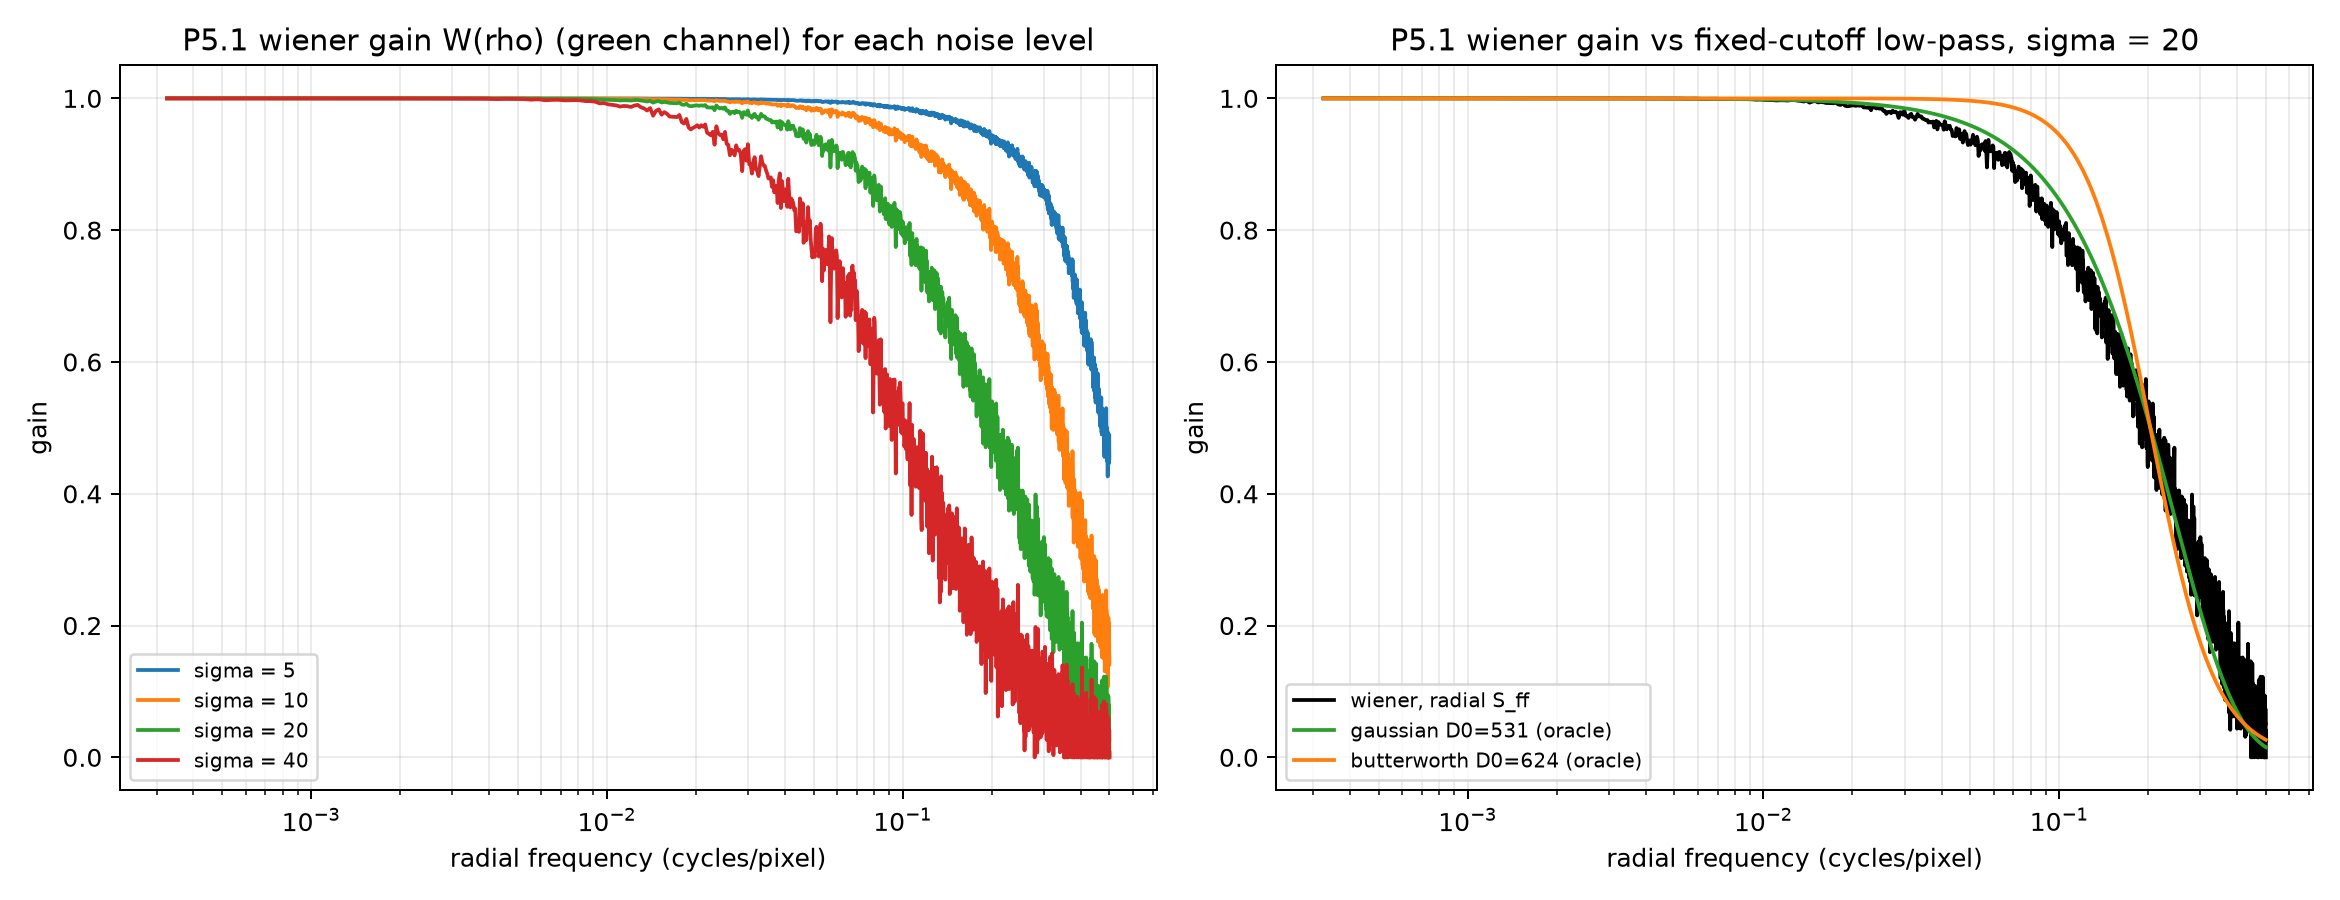
\includegraphics[width=0.95\linewidth]{problem_5/wiener_gain.png}
\caption{Left: the estimated Wiener gain (green channel) against radial frequency
for each $\sigma$. Right: at $\sigma=20$, the Wiener gain against the oracle-tuned
low-pass filters.}
\label{fig:gain}
\end{figure}

\paragraph{How the shrinkage behaves.} $W=1/(1+S_{nn}/S_{ff})$ depends only on the
local signal-to-noise ratio at each frequency. Natural-image power falls steeply
with frequency while white noise is flat, so $W$ stays near 1 at low frequencies,
where the image dominates, and falls towards 0 where the image power drops below
the noise. When $\sigma$ grows, $S_{nn}$ rises at every frequency and the crossover
moves down (Fig.~\ref{fig:gain}, left; \code{wiener\_gain.txt}): the gain at 0.1
cycles/pixel is 0.985 at $\sigma=5$ and 0.510 at $\sigma=40$, and the frequency where
it falls to one half drops from 0.470 to 0.088 cycles/pixel. A fixed-cutoff low-pass filter has the
same general shape, but its cutoff and roll-off are fixed in advance and have to be
tuned to each noise level and image. The Wiener gain sets its own shape from the
measured spectrum, uses no reference, and its roll-off follows the image rather
than a formula. At $\sigma=20$ the oracle-tuned Gaussian ended up with almost the
same curve as the estimated Wiener gain (Fig.~\ref{fig:gain}, right), which is why
the two score 29.132 and 29.137 dB. Across all four noise levels the untuned radial
Wiener filter matches or beats the oracle-tuned low-pass filters, and the oracle
Wiener filter is about 1 dB higher still, which is the cost of estimating $S_{ff}$
from noisy data. The 2-D smoothed estimate is slightly better than the radial one
at low noise and worse at $\sigma=40$ (SSIM 0.5925 against 0.6216). A
$15\times15$ box averages far fewer periodogram values than a full ring, and where
$S_{ff}$ is close to $S_{nn}$ the subtraction amplifies that extra variance into
patches of frequencies where noise is let through.

Wiener does not win every comparison. The oracle-tuned bilateral filter beats the
radial Wiener filter at every $\sigma$ (by 1.8 dB at $\sigma=5$ and 0.4 dB at
$\sigma=40$), and beats even the oracle Wiener filter for $\sigma\le20$. Wiener's
optimality is among \emph{linear} estimators, under second-order statistics of a
stationary model; the bilateral filter is nonlinear and adapts its averaging at
every pixel. In fairness, the bilateral result had two parameters tuned against the
clean image, while the radial Wiener filter used only $\sigma$.

\begin{figure}[H]
\centering
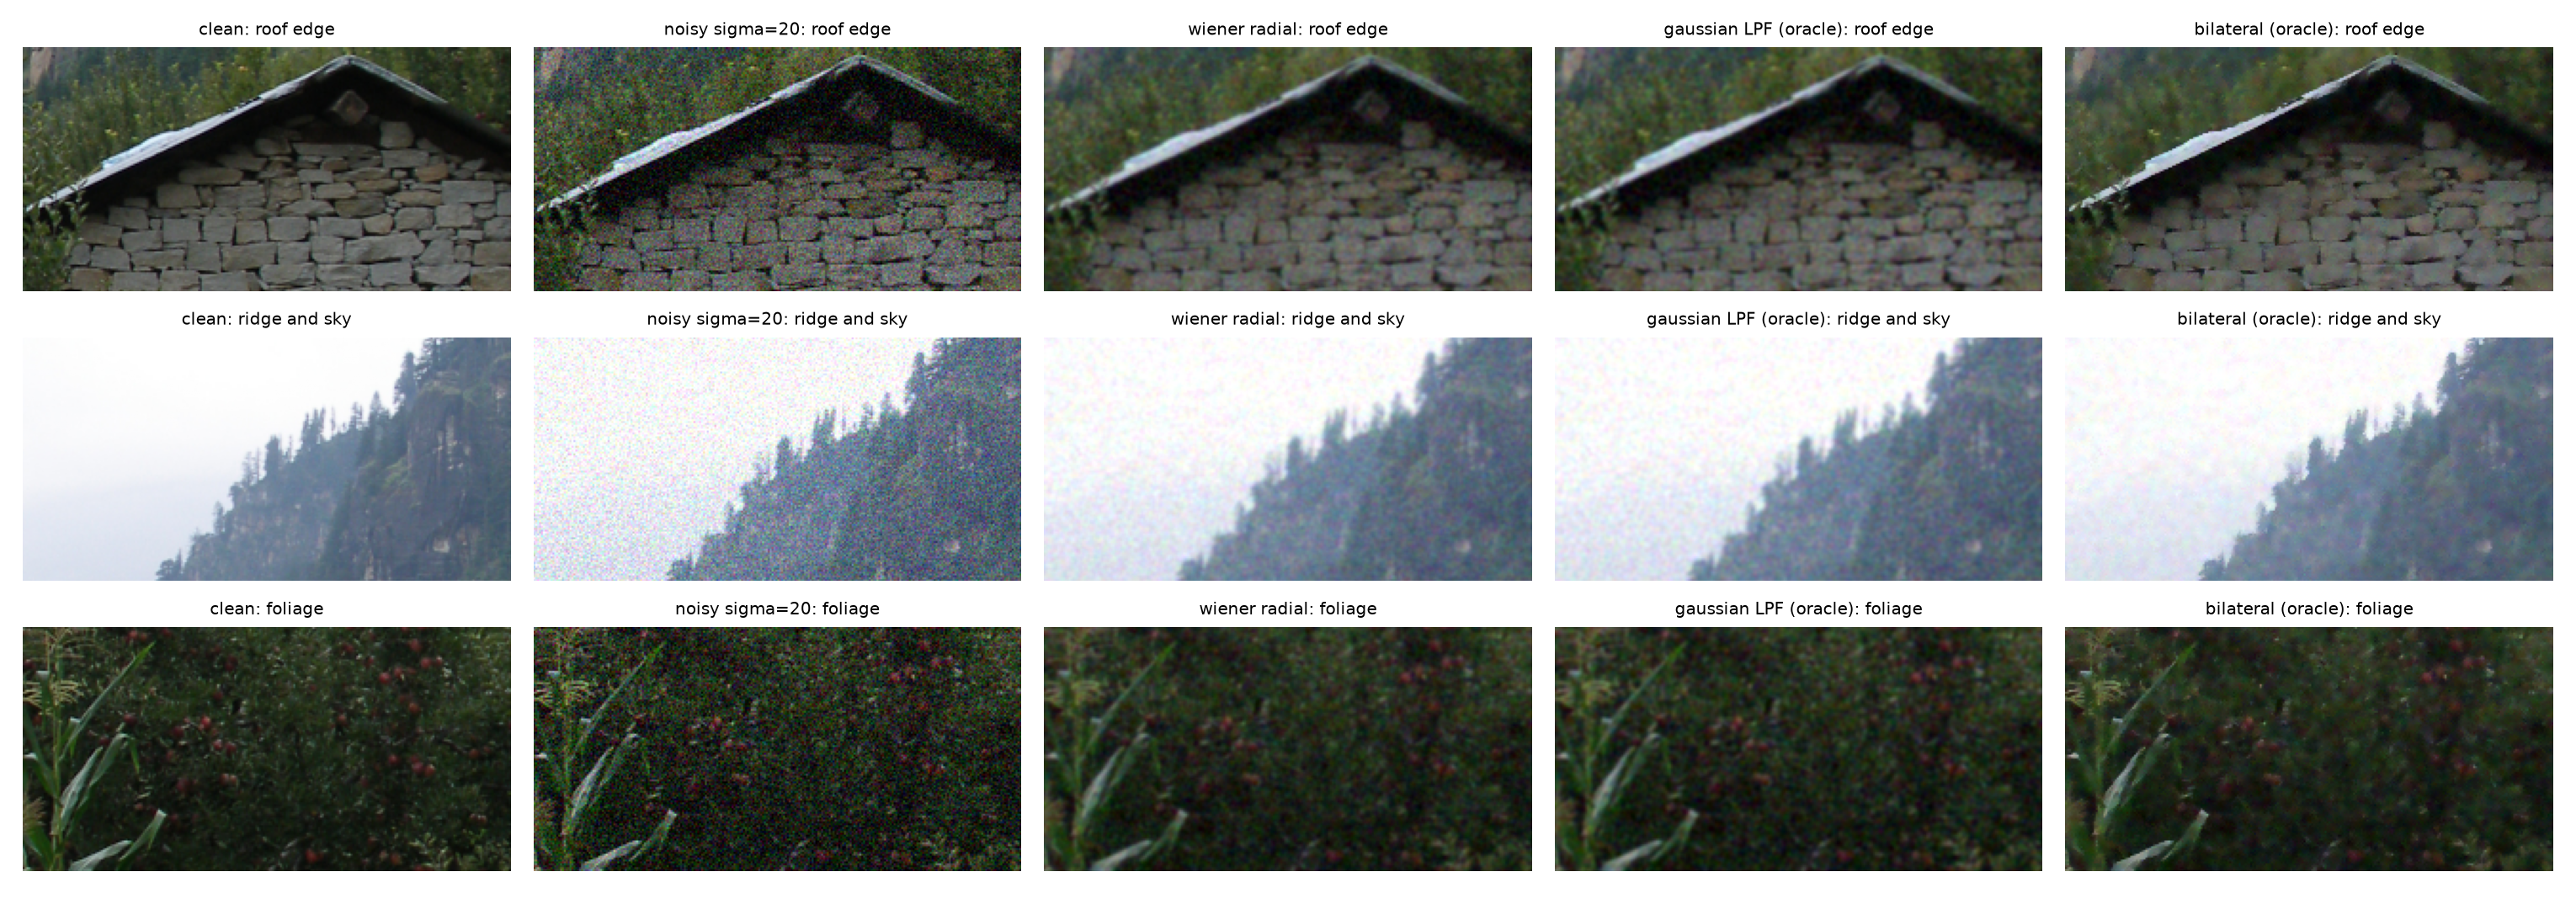
\includegraphics[width=\linewidth]{problem_5/denoising_crops.png}
\caption{Crops at $\sigma=20$: roof edge, ridge against sky, foliage.}
\label{fig:denoise-crops}
\end{figure}

\subsection{Testing the assumptions}

\paragraph{Mis-specified noise power.} At $\sigma=20$ the radial Wiener filter was run
assuming noise power $0.5S_{nn}$, $S_{nn}$ and $2S_{nn}$, with $\hat S_{ff}$
re-estimated each time as a user of the filter would. The error is split into a
flat band (the 50\,\% of pixels with the smallest clean-image gradient) and an edge
band (the largest 10\,\%), in 8-bit levels.

\begin{table}[H]
\centering
\begin{tabular}{rrrrrr}
\toprule
assumed & PSNR (dB) & SSIM & flat RMSE & edge RMSE & mean gain\\
\midrule
$0.5S_{nn}$ & 26.389 & 0.5633 & 11.533 & 13.959 & 0.5980\\
$S_{nn}$ & 29.137 & 0.7373 & 6.910 & 14.987 & 0.1992\\
$2S_{nn}$ & 27.644 & 0.7038 & 6.767 & 20.257 & 0.0473\\
\bottomrule
\end{tabular}
\caption{Noise-power mis-specification at $\sigma=20$ (\code{misspecification.txt}).}
\label{tab:misspec}
\end{table}

With the subtraction estimate, the gain is $W=1-\alpha S_{nn}/\overline{|G|^2}$
(floored at 0) for an assumed power $\alpha S_{nn}$. At high frequencies, where
$\overline{|G|^2}\approx S_{nn}$ (pure noise), the correct filter gives
$W\approx0$, but $\alpha=0.5$ gives $W\approx0.5$, so half of the noise amplitude
there passes through. The mean gain triples, the flat-region error rises from 6.9 to
11.5 levels, and residual noise is visible everywhere (\code{misspecification.png}).
With $\alpha=2$ every frequency whose power is below twice the noise is removed,
including the frequencies that carry fine edges. The flat error barely changes
(6.77), but the edge error rises from 15.0 to 20.3 and the image looks smoothed. The
two failures are not symmetric: underestimation leaves noise where the image is
flat, overestimation blurs where it is not.

\paragraph{Why a correct Wiener filter still blurs edges.}

\begin{table}[H]
\centering
\begin{tabular}{lrrr}
\toprule
Method ($\sigma=20$) & flat RMSE & edge RMSE & edge / flat\\
\midrule
noisy input & 18.016 & 19.697 & 1.09\\
Wiener, radial & 6.910 & 14.987 & 2.17\\
Wiener, oracle & 6.382 & 12.401 & 1.94\\
Gaussian LPF (oracle-tuned) & 6.961 & 14.911 & 2.14\\
bilateral (oracle-tuned) & 5.935 & 12.009 & 2.02\\
\bottomrule
\end{tabular}
\caption{Where the remaining error sits (\code{edge\_blur.txt}).}
\label{tab:edge-blur}
\end{table}

Even with the correct noise power, the Wiener filter's error at edges is more than
twice its error in flat regions (Table~\ref{tab:edge-blur}), and the roof-edge profile
(\code{edge\_profile.png}) shows the bright roof line flattened from a luminance of
0.758 to 0.495 (0.567 even with the oracle spectrum), while the bilateral filter
keeps it at 0.770. The filter is linear and shift-invariant, so one gain $W(u,v)$ applies at every
pixel. $S_{ff}$ is an average over the whole image, which is mostly smooth
foliage, sky and mountain, so at high frequencies it is small and $W$ cuts them.
An edge is a local event whose energy is spread over all frequencies, including
those high ones, so it loses them too, even though near the edge the local signal
power at high frequency is far above the noise. MMSE optimality only promises the
smallest mean squared error averaged over the image and over the noise, among linear
filters, for a stationary model described by its second-order statistics. It does
not promise small error at any particular place, and edges are a small fraction of
the pixels, so the average can be minimised while they are blurred. A natural
image is not a stationary Gaussian field: its edges are sparse and localised. A
nonlinear filter that looks at local intensities, such as the bilateral filter,
achieves both lower flat and lower edge error here (5.9 and 12.0).

\paragraph{Real noisy photograph: blocked.} This part needs a genuinely noisy
photograph taken by the student, and none had been supplied when this report was
produced (\code{real\_noise.txt} records the blocked run). The case study is
implemented and runs automatically once a file named \code{noisy*} is placed in
\code{photos/}. It estimates $\sigma$ per channel with Immerkær's method \cite{immerkaer}, applies the
white-noise radial Wiener filter at full resolution, and compares crops, residuals,
residual spectra, residual autocorrelation and residual level against brightness
with a synthetic white-noise case at the same $\sigma$, without PSNR or SSIM. The
noise estimator was validated on the synthetic images: injected $\sigma$ of 5, 10, 20
and 40 are estimated as 5.895, 10.531, 20.278 and 40.125, and the clean reference
itself gives 2.540, the floor set by fine image texture and the reference's own
noise. Real camera noise is expected to depart from the white-noise model in four
ways the analysis is built to show: shot noise makes its variance depend on
brightness, demosaicing correlates neighbouring pixels and colours, in-camera
sharpening boosts its high frequencies, and JPEG compression removes some of them
in $8\times8$ blocks.

\paragraph{Conclusion.} The Wiener gain adapts its cut-off to the measured spectrum
and the noise level, and without any tuning it matches low-pass filters tuned on the
clean image. Its optimality is limited to linear filters under a stationary model:
it blurs edges even when the noise power is right, it degrades in opposite ways
when the noise power is wrong, and a tuned nonlinear filter beat it here.
